\documentclass[a4paper,10pt]{report}
\usepackage[utf8]{inputenc}

% Title Page
\author{Łukasz Adamowicz}

\usepackage{mathcommands}
\usepackage{amsthm}
\usepackage{algorithm}
\usepackage{algpseudocode}
\usepackage{hyperref}
\usepackage{graphicx}
\newtheorem{theorem}{Theorem}
\newtheorem{statement}{Statement}
\newtheorem{lemma}{Lemma}
\newtheorem{remark}{Remark}
\renewcommand{\thesection}{\arabic{section}}
\begin{document}
% \maketitle
\begin{titlepage}
    \begin{center}
        \textbf{\Large Title of Your Internship}\\[2cm]
        \textbf{Academic Year:} 2024--2025\\
        \textbf{Master's Program:} M2 Mathématiques, Modélisation et Apprentissage\\
        \textbf{Name:} Łukasz Adamowicz\\[1cm]
        \textbf{Internship Supervisor:} Professor Fred Hamprecht\\
        \textbf{Email:} fred.hamprecht@iwr.uni-heidelberg.de\\[1cm]
        \textbf{Hosting institution:}\\
        Heidelberg University,\\
        Interdisciplinary Center for Scientific Computing\\
        \textbf{UFR Contact:}\\
        Alexis Glaunes\\
        alexis.glaunes@parisdescartes.fr\\[2cm]

        % Optionally add logos, date, etc.
        \vfill
        \today
    \end{center}
\end{titlepage}


\begin{abstract}
TK make sure every equation is numbered

During my internship at Hamprecht Lab I investigated training deep learning models using loss function that's defined in an implicit way.
The goal of the internship was to adapt and implement the approach from  preprint \cite{neuralscf} to ...different setting. This required ...

I implemented two approaches and resolved stability issue
\end{abstract}


\tableofcontents
\newpage
\section{Lab presentation}
SciAi groups research focus is on ...
The goal is to approximate energy functional...
This would allow for computation of ... in complexity O(n) instead of ...
TK
We assume $E(\theta, p)$ is ??? differentiable/continuous

Electron density is approximated by a set of finite-dimensional  atom-centered function
What is important is finding fixed point of the model , which should approximate the ground state $p_{gs}$.
Since ground state is not always known, the model should converge to ground start from wide range of starting points.

\begin{equation}
 \rho(r) = \sum_{i=1}^n p_i \Omega_i(r)
\end{equation}

\begin{equation}
 w_i = \int_{\R^3} \Omega_i(r)dr
\end{equation}

Representation of electron density
\newpage
\section{Carried out work}
Notation: Let $E(\theta, M ,p)$ denote the energy model, with $\theta \in \R^k$ being model parameters, $M$ the molecule and $p=(p_1, \ldots ,p_n )\in \R^n$ density coefficients. Vector $w$ corresponds to
By $\frac{d}{d\theta}$ we mean total derivative, while $\pd{}{\theta}$ denotes partial derivative with respect to argument $\theta$.

TK $p$ DIMENSION DEPENDS ON N $M$
TK WHAT IS THE DIMENSION OF p?



 \subsection{Goal of the project}
1. Implicit funciton theorem

The goal of the project was to investigate and minimize the following loss
\begin{equation}\label{bilevel}
 \min_\theta \sum_i \mathcal{L}(p_{\theta}^{M_i}),
\end{equation}
where
\begin{equation}
  p_\theta^{M_i}:=\argmin_{p : \inner{w}{p}=N_i} E(\theta,M_i,p)
\end{equation}
and $\mathcal{L}_{M_i}(p) = \frac{1}{2}\mse{p-p_{M_i}}$ is the standard $L_2$ loss.

In the rest of the report I will drop index $M_i$. This will notably simplify the notation.
Therefore I will write $E(\theta,p)$ instead of $E(\theta,M,p)$ and the same for $p_\theta$, $\mathcal{L}(p)$ and so on.
The quantity $\pth$ is a \textbf{fixed point}.
This falls under the domain of \textbf{bilevel optimization}.

The main problem lies in computing the gradient of $\mathcal{L}(p_\theta)$


\subsubsection{One molecule}
Let $w$ be a non-zero vector and $N>0$ a positive number.
We consider the problem of minimizing

\begin{equation}
 \min_\theta \mathcal{L}(p_\theta),
\end{equation}
with
\begin{equation}
\pth = \argmin_{\substack{p \in \R^n \\ p: \inner{p}{w}=N }} E(\theta, p)
\end{equation}
and
\begin{equation}
 \mathcal{L}(p) = \frac{1}{2} \norm{p-p_{gs}}^2,
\end{equation}
where $p_{gs}$ are ground state density coefficiens given by the data and satisfy the constraint $\inner{p_{gs}}{w} = N$.


\subsubsection{Direct approach}
The most direct approach would be to backpropagate through the trajectory of the fixed point. More precisely, given
\subsection{Implicit function theorem}
This can be accomplished by using implicit function theorem

TK ADD STATEMENT
I use the version of implicit function theorem from \cite{zucchet2022beyond}, which in turn is taken from \cite{dontchev2009implicit}.
\begin{theorem}[Implicit Function Theorem, \cite{zucchet2022beyond} ]
Let $G(\theta, p): \R^k \times \R^n \to \R^n$ be $C^1$ and $(\bar{\theta}, \bar{p})$ such that $G(\bar{\theta},\bar{p})=0$. If the jacobian
$\pd{G}{p}(\bar{\theta},\bar{p})$ is non-singular, then there exists an open neighbourhood $U$ of $\bar{\theta} $ and a function $p(\theta):U \to \R^n$, such that $G(\theta, p(\theta)) = 0$. Moreover $p(\theta)$ is also differentiable with
the  derivative given by
\begin{equation}
\pd{p}{\theta}= - \bigg(\pd{G}{p}(\theta, p(\theta))\bigg)^{-1} \frac{\partial^2 G}{\partial \theta \partial p}(\theta, p(\theta)).
\end{equation}

\end{theorem}
In our case $G = \pd{E}{p}$. Since our model is $C^1$/smooth with respect to  arguments and the hessian of $E$ is ...

\subsubsection{Basis dependent approach}
TK find better notation

First, let's consider the problem in an orthogonal basis containing $w$.
Let the basis be $(e_1,\ldots, e_{n-1}, w)$.
Let $\widetilde{E}(\theta, p) = E(\theta, p_{gs}+ p)$ and $p = \sum_{i=1}^{n-1} p_i e_i$.
Then $\widetilde E(\theta, \cdot)$ is just $E$ restricted to affine space $p_{gs}+\text{ span} (w)^\perp$
and the problem becomes
\begin{equation}
  \min_\theta \mathcal{L}(p_\theta),
\end{equation}


\begin{equation}
 \pth = \argmin_{p\in \R^{n-1}} \widetilde{E}(\theta, p)
\end{equation}


TK CHECK NOTATION FOR HESSIAN AND MIXED DERIVATIVE
TK CHANGE symbol for A
\begin{statement}
The gradient of $\mathcal{L}(\pth)$ is equal to
 \begin{equation}
 \dth{\mathcal{L}(\pth)} = -(\pth - p_{gs}) \bigg(\frac{\partial \nabla_p \widetilde{E}}{\partial p}\bigg)^{-1}  \frac{\partial  \nabla_p \widetilde{E}}{\partial \theta}
\end{equation}
\end{statement}

To obtain the gradient of the loss we start from chain rule
\begin{equation}
 \dth{\mathcal{L}(\pth)} = \pd{\mathcal{L}}{p}\dth{\pth}.
\end{equation}
Since $\pd{\mathcal{L}}{p}(\pth )= \pth-p_{gs}$ all we need to find is $\dth{\pth}.$
% General formula



\begin{statement}
The gradient of $\pth$ is equal to
 \begin{equation}
   \dth{\pth} = -\bigg(\frac{\partial  \pd{\widetilde{E}}{p}  }{\partial p}\bigg)^{-1} \pd{\nabla_p \widetilde{E}}{\theta}(\theta, \pth)
 \end{equation}
\end{statement}

\begin{proof}
By definition $\widetilde{E}(\theta, \cdot)$ attains its minimum at $\pth$ it follows that
\begin{equation}
\pd{\widetilde{E}}{p}(\theta, \pth) = 0.
\end{equation}

TK correct the formula by adding gradient
By taking derivative with respect to $\theta$, we get


% total derivative
\begin{equation}
0=\dth{}\bigg(\pd{  \nabla_p \widetilde{E}   }{p}(\theta, p_\theta)\bigg) = \pd{ \nabla_p \widetilde{E}  }{\theta} + \pd{ \nabla_p \widetilde{E}  }{p} \dth{\pth}.
\end{equation}
Therefore
\begin{equation}
 \dth{\pth} = -\bigg(\frac{\partial \nabla_p \widetilde{E}}{\partial p}\bigg)^{-1} \pd{\nabla_p \widetilde{E}}{\theta}(\theta, \pth).
\end{equation}

Let's denote the hessian of $\widetilde{E}$ as

\begin{equation}
 H := \bigg(\frac{\partial \nabla_p \widetilde{E}}{\partial p}\bigg)(\theta,\pth) = H_{\widetilde{E}}(\theta,\pth)
\end{equation}
\end{proof}
This gives us the final formula
\begin{equation}
 \dth{\mathcal{L}(\pth)} = - (\pth - p_{gs}) H^{-1}  \frac{\partial \nabla_p \widetilde{E}}{\partial \theta}\bigg|_{p=p_\theta, \theta=\theta}.
\end{equation}


% Following \cite{neuralscf} we denote
% \begin{equation}
%  y = -(\pth-p_{gs})A^{-1}.
% \end{equation}
% The final gradient formula is
% \begin{equation}
%  \dth{\mathcal{L}(\pth)} = y \cdot \frac{\partial \nabla_p \widetilde{E}}{\partial \theta}\bigg|_{p=p_\theta, \theta=\theta}.
% \end{equation}



TK Maybe put somewhere else
The quantity $\frac{\partial \nabla_p E}{\partial \theta}$ is obtained using automatic differentation and $y$ is a solution to linear system $yA = -(\pth-p_{gs})$. Solving for $y$ is done using matrix-free methods such as conjugate gradient method or plain gradient descent on square error loss $\mse{yA + \pth+p_{gs}}$ since $yA$ is vector-jacobian product, which also can be evaluated efficiently using automatic differentation. Since $E$ is ..., and a approximation of physical potential function, it's reasonable to assume that it is positive-definite.

% END OF basis approach
\subsubsection{Basis-free approach}

Since it's more natural to implement the algorithm


\subsubsection{Derivation of the gradient}
 To this end we make use of the following lemma.

\begin{lemma}
 Let $P := Id -\frac{ww^T}{w^Tw} $ be the projection operator onto subspace $V = \text{span}(w)^{\perp}$. Then the following equality is true
 \begin{equation}
  P\big(\nabla_p E(\theta, p_\theta)\big) = 0
 \end{equation}

\end{lemma}

\begin{proof}
  Since $p_\theta$ is the minimum of $E(\theta,p)$ restricted to $V$ we have \[\langle \nabla_p E(\theta,p_{\theta}), u \rangle = 0\] for any $u\in V$. Taking $u = P\big( \nabla_p E(\theta,p_\theta)\big)$ we obtain
  \[\langle \nabla_p E(\theta,p_{\theta}), P\big( \nabla_p E(\theta,p_\theta)\big) \rangle = \norm{P\big( \nabla_p E(\theta,p_\theta)\big)}^2=0,\]
  which conludes the proof.
\end{proof}

Let's denote $F(\theta,p) :=P (\nabla_p E(\theta,p)).$ Then the previous condition can be written as
\begin{equation}
 F(\theta,p_\theta) = 0.
\end{equation}
We take the derivative with respect to $\theta$
\begin{equation}
0=\dth{F(\theta, p_\theta)} = \pd{F}{\theta} + \pd{F}{p} \dth{\pth}.
\end{equation}
Rearranging we obtain
\begin{equation}
 \frac{d p_\theta}{d\theta} = - \bigg(\frac{\partial F}{\partial p}\bigg)^{-1}  \frac{\partial F}{\partial \theta}\bigg|_{p=p_\theta, \theta=\theta}.
\end{equation}

Therefore the full gradient of $\mathcal{L}(\pth)$ is equal to
\begin{equation}
 \dth{\mathcal{L}(\pth)} = - (\pth - p_{gs})\bigg(\frac{\partial F}{\partial p}\bigg)^{-1}  \frac{\partial F}{\partial \theta}\bigg|_{p=p_\theta, \theta=\theta}.
\end{equation}
\begin{remark}
 The jacobian $\frac{\partial F}{\partial p}$ is not invertible, since $F$ is a projection.
 \begin{equation}
  F(\theta, p) = \sum_{i=1}^{n-1} \inner{\nabla_p E(\theta, p)}{e_i} e_i +  0 \cdot w
 \end{equation}

 The jacobian matrix in the basis $(e_0,...,e_{n-1},w)$ can be written as \begin{equation}
                      \frac{\partial F}{\partial p}\bigg|_{p=\pth} =\begin{bmatrix}
H & 0 \\
0 & 0
\end{bmatrix}.
                     \end{equation}



The solution to linear regression
\begin{equation}
 y = \underset{u\in \R^n}{\mathrm{argmin }}\bigg\|u \begin{bmatrix}
H & 0 \\
0 & 0
\end{bmatrix} + (p_\theta-p_{true})\bigg\|^2
\end{equation}
is satisfied for by $y$ of the form

TK RESOLVE DIMENSIONALITY NOTATION PROBLEMS. IS $P:R^n ->R^n-1$ or does is just put zero on the last component?
\begin{equation}
 y = P\big((\pth-p_{gs})\big)H^{-1} + \alpha w.
\end{equation}
Since $F$ is a projection onto plane perpendicular to $w$, it shouldn't matter which $y$ we choose.
That is to say
\begin{equation}
 \inner{y}{ \pd{F}{\theta}}=\inner{Py}{\pd{F}{\theta}}.
\end{equation}

Therefore, the formula doesn't change, however some algorithms for solving linear systems might not work, if they rely on invertibility.
\end{remark}

We can rewrite the formula for the gradient as
\begin{equation}
 \dth{\mathcal{L}(\pth)} = y \cdot  \frac{\partial F}{\partial \theta}\bigg|_{p=p_\theta, \theta=\theta}.
\end{equation}

We can treat $y$ as constant vector and pull it inside partial derivative to obtain


\begin{equation}
 \dth{\mathcal{L}(\pth)} =   \frac{\partial (\inner{y}{F})}{\partial \theta}\bigg|_{p=p_\theta, \theta=\theta}.
\end{equation}

% To make $y$ unique we add a term such as $\inner{u}{w}^2$ or add additional constraints.


The whole procedure for gradient calculation is as below
\begin{algorithm}[H]
\caption{Gradient Calculation}
\begin{algorithmic}[1]
\Require Data $p_{gs}$, model parameters $\theta$
\State  Solve for $p_\theta$ such that $F(p_\theta, \theta) = 0$
\State Solve for $y = \underset{u\in \mathbb{R}^n}{\mathrm{argmin}} \bigg\|u \frac{\partial F}{\partial p}\bigg|_{p=p_\theta} + (p_\theta-p_{gs})\bigg\|^2$
\State Compute gradient $\dth{\mathcal{L}(\pth)} = \frac{\partial (\inner{y}{F})}{\partial \theta}\bigg|_{\substack{p=p_\theta \\\theta= \theta}}$
\State \Return $\dth{\mathcal{L}(\pth)}$
\end{algorithmic}
\end{algorithm}

The implementation details, such as root-solver, are described in \ref{sec:impl}.



3. Lagrangian approach?

TK COME BACK WHEN YOU ACTUALLY DO IT BY HAND
 \begin{equation}
\min_{\lambda,\theta} L
 \end{equation}

5. Error analysis for both approximate fixed point and solving linear equation
TK add section from Sacramento,Zuccheti
\subsection{ Equilibrium propagation}

\subsubsection{Base version}
During my internship I also implemented and tested optimization using Equilibrium Propagation (see \cite{eqprop}, \cite{zucchet2022beyond}), which is an alternative method of computing the gradient with respect to model parameters.
Let's denote
\begin{equation}
H(\theta, p, \beta) := \beta \mathcal{L}(p) + E(\theta, p),
\end{equation}
where $\beta \in \R$.
 This is called \textbf{total energy} in \cite{eqprop}. Let's also denote
\begin{equation}
p_{\theta}^{\beta}:=\argmin_p H(\theta, p, \beta)
\end{equation}
\begin{remark}
 For $\beta>0$ the function $p \mapsto \beta \mathcal{L}(p)$ is strongly convex, so $H$ has ... TK HOW TO WRITE should converge better

 Since $H(\theta,p,0) = E(\theta,p)$ we have $p_{\theta}^{0}=p_{\theta}$.
 \end{remark}





\begin{statement}[Equilibrium propagation formula]
 \begin{equation}
 \frac{d}{d\theta} \mathcal{L}(p_\theta) = \lim_{\beta \to 0} \frac{\pd{H}{\theta}(\theta, p_\theta^\beta, \beta)-\pd{H}{\theta}(\theta, p_\theta^0, 0) }{\beta} = \lim_{\beta \to 0}\frac{1}{\beta} \pd{}{\theta} \bigg(H(\theta, p_\theta^\beta,\beta) - H(\theta, p_\theta^0, 0)\bigg).
\end{equation}
\end{statement}
This formula can be used to numerically approximate the gradient of the loss function.
Since in our case $\mathcal{L}(p)$ doesn't depend on $\theta$, $\pd{H}{\theta}$ simplifies to $\pd{E}{\theta}$, although the formula remains true is $\mathcal{L}$ is also a function of $\theta$. For example there might be regularization term added to $\mathcal{L}(p)$.

\begin{proof} Let's denote
 \begin{equation}
 G(\theta, \beta) := H(\theta, p_\theta^\beta, \beta).
\end{equation}
Because $p_\theta^\beta$ is $C^2$, $G$ is $C^2$ and so we have the symmetry of second derivatives
\begin{equation}
 \frac{d}{d\theta}\frac{d}{d\beta}G(\theta,\beta)\big|_{\beta=0, \theta = \theta} =\frac{d}{d\beta}\frac{d}{d\theta}G(\theta,\beta)\big|_{\beta=0, \theta = \theta}
\end{equation}
We have

\begin{equation}\label{eqcond}
 \frac{dG}{d\beta} = \frac{\partial H}{\partial \beta} + \frac{\partial H}{\partial p}(\theta,\pthb, \beta)\frac{\partial \pthb}{\partial \beta}.
\end{equation}
By definition
\begin{equation}
\frac{\partial H}{\partial p}(\theta,\pthb, \beta)=0.
\end{equation}
The second term vanishes, leaving us with
\begin{equation}\label{pvanish}
  \frac{dG}{d\beta}\big|_{\beta=0} = \frac{\partial H}{\partial \beta}(\theta, \pth, 0)=\mathcal{L}(\pth).
\end{equation}
Analogically
\begin{equation}\label{thvanish}
 \frac{dG}{d\theta}=\frac{\partial H}{\partial \theta}(\theta, \pthb, \beta).
\end{equation}

TK Explain, why it's different iwe we switch back the order of derivatives.
In the end we obtain
\begin{align}
 \frac{d}{d\theta} \mathcal{L}(p_\theta) &=\frac{d}{d\theta}\frac{d}{d\beta}G(\theta,\beta)\big|_{\beta=0} = \frac{d}{d\beta}\frac{d}{d\theta}G(\theta,\beta)\big|_{\beta=0}=\\
 &=\lim_{\beta \to 0}\frac{1}{\beta} \pd{}{\theta} \bigg(H(\theta, p_\theta^\beta,\beta) - H(\theta, p_\theta^0, 0)\bigg)
\end{align}

\end{proof}

\begin{remark}
 It turns out the formula remains the same if we change the fixed point definition to
\begin{equation}
 p_\theta^\beta = \argmin_{\substack{p \in \R^n \\ p: \inner{p}{w}=N }} H(\theta, p, \beta)
\end{equation}
In this case equilibrium condition \ref{eqcond} changes to
\begin{equation*}
P\bigg(\frac{\partial H}{\partial p}(\theta,\pthb, \beta)\bigg)=0,
\end{equation*}
where, as before, $P$ is a projection operator. Since $\inner{w}{\pthb}$ is does not depend on $\beta$ nor $\theta$ both \ref{pvanish} and \ref{thvanish} also stay the same and so the final formula remains unchanged.

\end{remark}


\begin{algorithm}[H]
\caption{Equilibrium propagation }
\begin{algorithmic}[1]
\Require Data $p_{gs}$, model parameters $\theta$, $\beta>0$.
\State  Solve for $p_\theta$ such that $F(p_\theta, \theta) = 0$
\State Solve for $y = \underset{u\in \mathbb{R}^n}{\mathrm{argmin}} \bigg\|u \frac{\partial F}{\partial p}\bigg|_{p=p_\theta} + (p_\theta-p_{gs})\bigg\|^2$
\State Compute gradient $\dth{\mathcal{L}(\pth)} = \frac{\partial (\inner{y}{F})}{\partial \theta}\bigg|_{\substack{p=p_\theta \\\theta= \theta}}$
\State \Return $\dth{\mathcal{L}(\pth)}$
\end{algorithmic}
\end{algorithm}


5. Error margins

\subsection{Results}
\subsubsection{Implicit function approach}
TK SPECIFY ITS ONE MOLECULE APPROACH
 For reasons yet unknown to me I have not been able to make jacobian approach work for the purpose of finetuning the model. Despite loss function decreasing during course of the training, density difference during density optimization run did not improve. This suggests, that jacobian approach did not in fact move the fixed point $\pth$ to real ground state $p_{gs}$ or did it while making energy landscape much more difficult to navigate.

 I tested the algorithm with various tolerance threshold on both projected gradient descent and linear equation solver.



 TK CREATE GRADIENT OF THE MODEL AND PUT HERE.
TK denop pictures
\subsubsection{assuming symmetric second derivative}

Hessian symmetry numerical check
\subsubsection{Convergence thresholds}
\subsubsection{Conjugate gradient}
I implemented and used conjugate gradient method for solving linear system. However, the algorithm rapidly diverged and proved to be unsuitable.

\subsection{Equilibrium propagation approach}
In contrast to jacobian approach I managed to finetune the model on single molecule.
The training loss decreased. What is much more important is that density difference also decreased, when root finding algorithm was run from a different starting point.

\begin{figure}[h!]
 \centering
 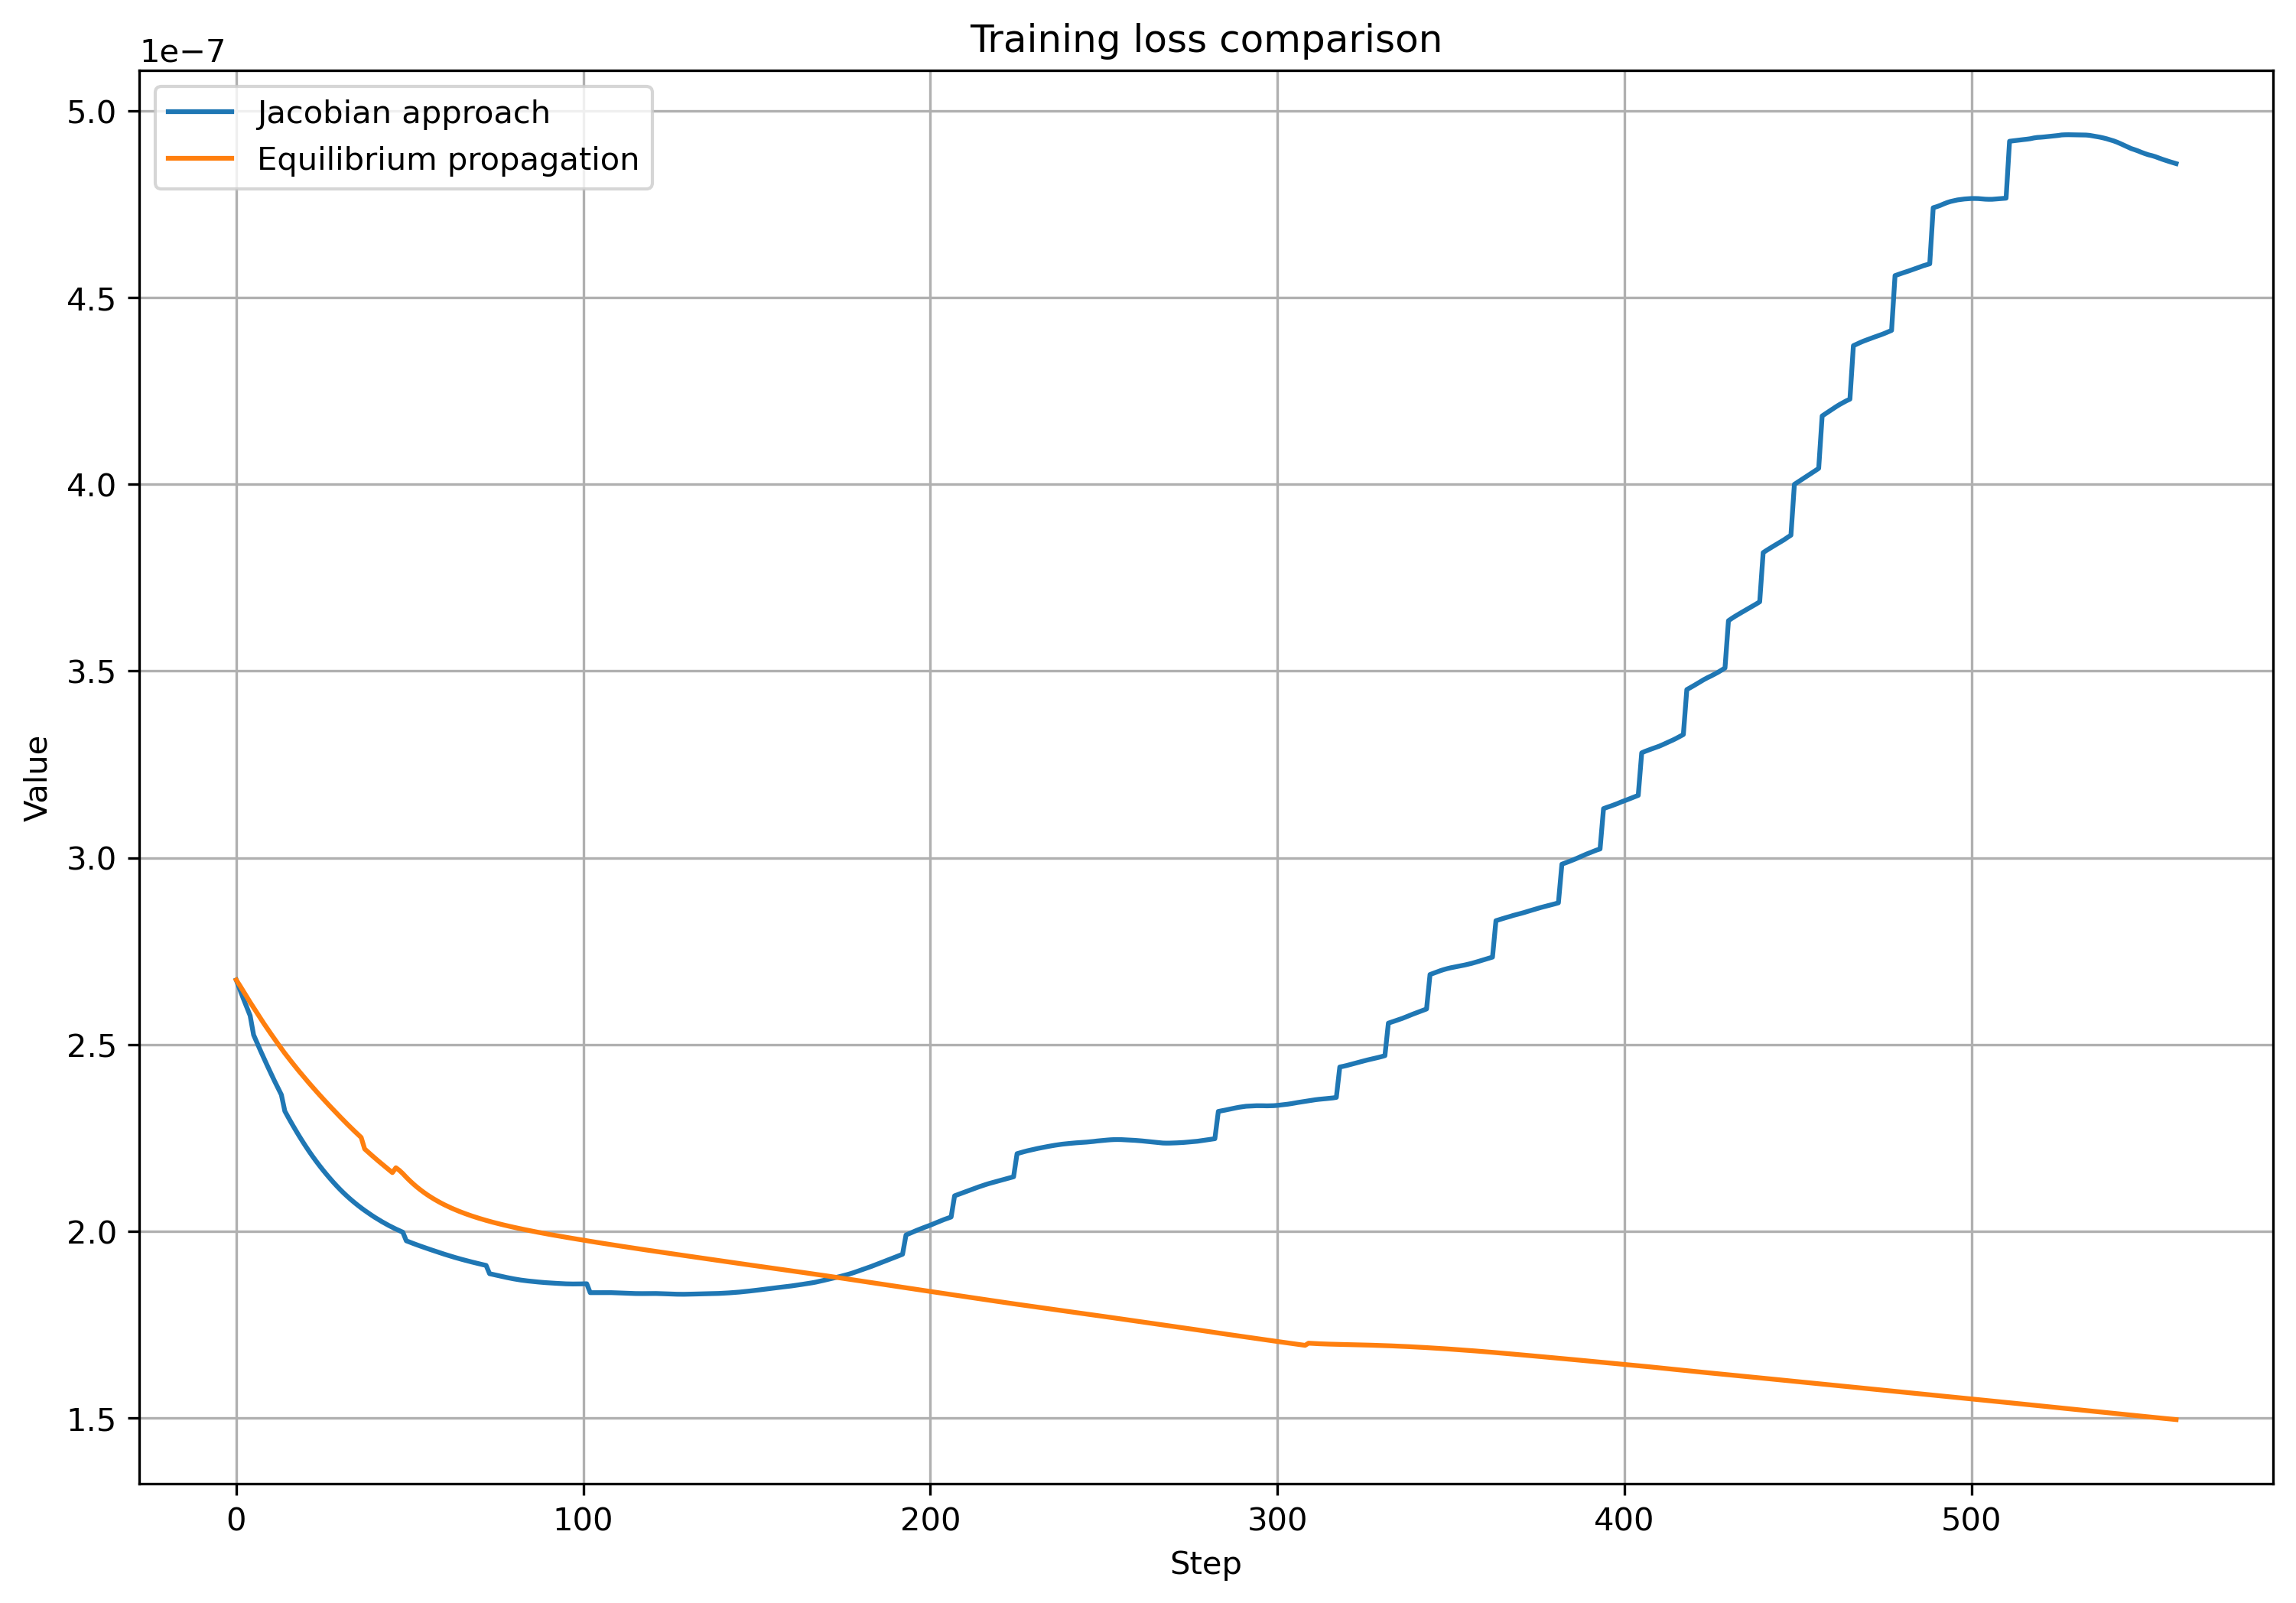
\includegraphics[scale=0.5]{images/loss_comparison.png}
 \caption{Comparison of training loss for jacobian and EP approaches.}
 % loss_comparison.png: 3002x2096 px, 300dpi, 25.42x17.75 cm, bb=0 0 720 503
\end{figure}


TK deno picture
\subsection{Stability issues}
Implicit loss training falls under the framework of deep equilibrium model (DEQ). One of the issues plaguing DEQ models is training stability. As training goes on, obtaining the fixed point takes longer and longer. This is reported in \cite{opticalflow}, \cite{bai2021stabilizing}, \cite{burger2025dequify} and \cite{geng2023torchdeq}.This was also the case for me when training multiple molecules. To alleviate the issue I adapted a technique introduced in \cite{opticalflow} called \textbf{fixed point correction}. I am not aware of any explanation why the technique works. It stabilizes the training. I am not aware of any explanation why the technique stabilizes training.


TK

TK create pictures of gradients of the model while trained-no implicit loss, diverged and stabilized for both eqprop and jacobian approach.
Run them on the same settings
\subsubsection{Training on more than one molecule}
After resolving stability issue I tested equilibrium propagation approach on a sample containing 180 and 1800 molecules taken from [name of the dataset, QMUGS or QM9]. I split the dataset in 80:10:10 ratios of train, validation and test, although test dataset ended up not being used. Regrettably, although train loss decreased, there was no improvement in validation loss and therefore no generalization.
TK put training loss and validation loss curves here.

\begin{remark}
 The problem \ref{bilevel} falls under \textbf{bilevel optimization}. However, due to memory and computational constraints the gradient is computed in mini-batches. It's possible, that \textbf{stochastic bilevel optimization} requires adaptation to make it work due to its nested structure or effect on variance of the gradient update.
\end{remark}
\newpage
\section{Conclusions}
During the course of my internship at Hamprech Lab I have implemented and tested two approaches to implicit loss calculations. I have found that jacobian approach was not viable for the model I used and did not results in any metric improvement.
However equilibrium propagation approach did decrease targeted metrics. I have also encountered grevious model training stability issues and after extensive literature search adapted the technique to my setting.
On more personal level I learned working with version control within group, to conduct literature search, acquired knowledge about
\nocite{*}
\bibliographystyle{plain}
\bibliography{references.bib}


\section{Appendices}



\appendix
% \appendixname{Proof of}
\section{Proof of implicit function theorem}

\section{Technical details}
architecture graph, training details (lr, optimizer, etc), rootfinind details.
Further experiments
fixed point correction for EMA and various p values.
\appendix
\section{Implementation details} \label{sec:impl}
0. Technical details
    architecture,
    model
    training
    etc
\subsection{Training}
\subsubsection{Gradient calculation}
Gradients are obtained using automatic differentation
The algorithm for finding fixed point is projected gradient descent. Its starting point was set to ground state $p_{gs}$.
TK ADD threshold details

Both vjp can be obtained efficiently using automatic differen in PyTorch, so naturally I preferred using matrix free methods.

\subsubsection{Fixed point correcion}\label{sec:fpc}
Fixed point correction is a technique for stabilizing DEQ training. The technique described in \cite{opticalflow}, \cite{geng2023torchdeq}
and \cite{burger2025dequify} is as follows. Given fixed point trajectory $p_0= p_{gs}, p_1,\ldots, p_T\approx  \pth $ we uniformly select $N$ intermediate points $p_{i_1}, p_{i_2}, \ldots , p_{i_N}=p_T$ and


\end{document}
